% !TEX root = ../Thesis.tex
\chapter{Introduction}

In today's interconnected digital landscape, software security has become a critical concern as applications handle increasingly sensitive data and operate in hostile environments. The discovery of security vulnerabilities before deployment is essential to prevent exploitation by malicious actors, yet traditional testing approaches often fail to comprehensively explore all possible execution scenarios, leaving potential vulnerabilities undiscovered.

Among program analysis techniques, symbolic execution has emerged as a particularly powerful approach for automated vulnerability discovery. Unlike traditional testing that executes programs with concrete input values, symbolic execution treats inputs as mathematical symbols and tracks how these symbols propagate through program computations. When encountering conditional branches, the symbolic execution engine explores multiple possible paths simultaneously, building a comprehensive map of program behaviors. This systematic exploration capability makes symbolic execution especially valuable for security analysis, as it can automatically generate test cases that reach deep program states and trigger complex vulnerabilities such as buffer overflows, integer overflows, and format string bugs.

\textbf{Challenges in Symbolic Execution.} Despite its theoretical power, symbolic execution faces a fundamental scalability challenge known as the path explosion problem. As program complexity increases, the number of possible execution paths grows exponentially, quickly overwhelming computational resources and rendering the analysis intractable for real-world software systems. Modern applications can generate millions of execution paths from relatively small input variations, making exhaustive analysis computationally prohibitive.

\begin{figure}[htbp]
    \centering
    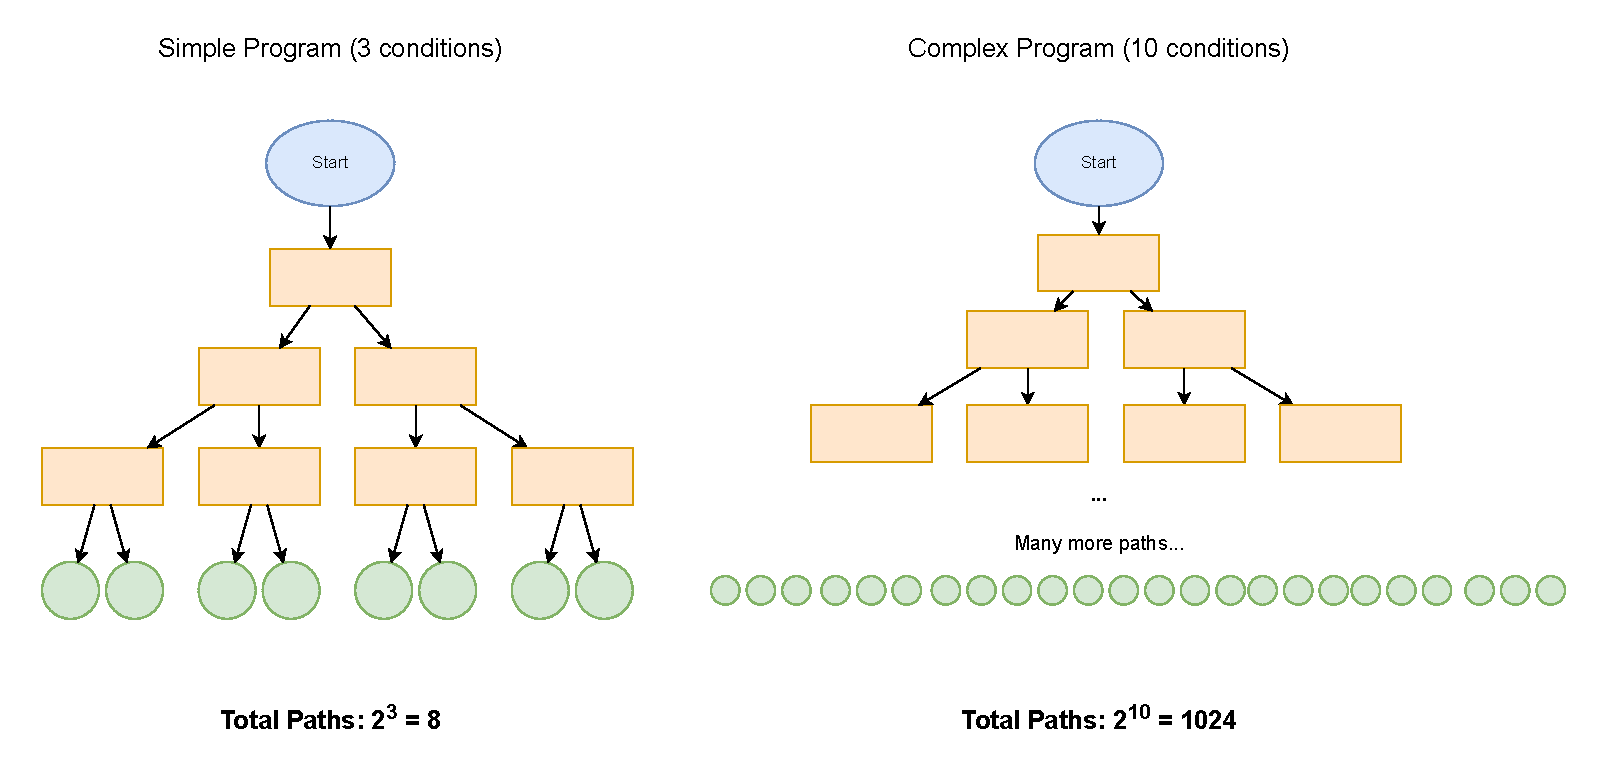
\includegraphics[width=\textwidth]{Figures/path_explosion_problem}
    \caption{Illustration of the path explosion problem: As program complexity increases from 3 to 10 conditions, the number of possible execution paths grows exponentially from 8 to 1024 paths.}
    \label{fig:path_explosion_problem}
\end{figure}

The path explosion problem is exacerbated by current symbolic execution engines that typically employ uniform exploration strategies, treating all program paths with equal priority regardless of their potential security relevance, as Figure~\ref{fig:path_explosion_problem} illustrates. This approach fails to recognize that paths processing user-controlled data are significantly more likely to contain vulnerabilities than paths handling only internal program state. Consequently, significant computational resources are often spent analyzing auxiliary program logic while security-critical paths that process external inputs receive no special attention.

Consider, for example, a network service that accepts client connections, reads incoming data via network sockets, performs input validation through multiple parsing layers, and eventually stores results using memory copy operations. Traditional symbolic execution would explore all execution paths with equal priority, including those that handle only internal configuration data or administrative functions that never process user input. A security-focused approach should recognize that paths flowing from network input through data processing to memory operations deserve higher priority due to their potential for buffer overflows, injection attacks, and other input-related vulnerabilities.

\textbf{Thesis Overview.} This work presents TraceGuard\footnote{https://github.com/ruben-hutter/TraceGuard}, an approach that integrates taint analysis with symbolic execution to enable intelligent path prioritization. Our methodology identifies and tracks data flow from critical sources such as user inputs, guiding the symbolic execution engine to focus computational resources on paths most likely to exhibit security-relevant behaviors.

The key insight driving this approach is that not all execution paths are equally valuable for security analysis—paths that interact with user-controlled data are significantly more likely to harbor vulnerabilities than those processing only internal program state. TraceGuard operationalizes this insight through a dynamic taint scoring mechanism that quantifies the security relevance of each symbolic execution state. By prioritizing states with higher taint scores, the symbolic execution engine directs its computational resources toward program regions most likely to contain security vulnerabilities, fundamentally transforming symbolic execution from an exhaustive search into a guided exploration strategy.

The main contributions of this thesis are:

\begin{itemize}
    \item \textbf{Taint-Guided Path Prioritization:} An integration of dynamic taint analysis with symbolic execution that uses taint propagation patterns to intelligently prioritize exploration of security-relevant execution paths.

    \item \textbf{Custom Angr Exploration Technique:} Implementation of\\ \texttt{TaintGuidedExploration}, a specialized exploration strategy that extends Angr's symbolic execution capabilities with security-focused path prioritization.

    \item \textbf{Function-Level Taint Tracking:} A comprehensive taint tracking system that monitors input functions, tracks taint propagation through function calls, and maintains detailed taint information throughout program execution.

    \item \textbf{Adaptive Scoring Algorithm:} A scoring mechanism that dynamically adjusts path priorities based on real-time taint analysis results, enabling the symbolic execution engine to focus computational resources on the most promising program regions.

    \item \textbf{Intelligent Function Hooking System:} A sophisticated hooking mechanism that intercepts function calls to analyze parameter taint status, allowing selective execution of only security-relevant code paths.

    \item \textbf{Practical Implementation and Validation:} A complete implementation using the angr symbolic execution framework, with comprehensive testing demonstrating the effectiveness of taint-guided exploration.
\end{itemize}

The effectiveness of this optimization is evaluated through controlled experiments comparing TraceGuard against standard Angr symbolic execution techniques using custom-designed test programs with known taint flow patterns. The evaluation examines key metrics including execution time, function call efficiency, and vulnerability detection reliability, with initial testing indicating significant improvements in analysis efficiency while maintaining comprehensive vulnerability detection capabilities.

This thesis focuses on binary program analysis using the angr symbolic execution framework, targeting user-space applications written in C/C++ and compiled for x86-64 architectures. The evaluation methodology centers on custom-designed test programs that demonstrate clear taint flow patterns, specifically crafted to evaluate TraceGuard's ability to distinguish between tainted and untainted execution paths.

The thesis is organized as follows:

\begin{itemize}
    \item \textbf{Chapter 2} provides essential background on symbolic execution, taint analysis, and the angr framework.
    \item \textbf{Chapter 3} surveys related work in symbolic execution optimization and taint analysis techniques.
    \item \textbf{Chapter 4} presents the conceptual framework and theoretical algorithms underlying TraceGuard's taint-guided exploration strategy.
    \item \textbf{Chapter 5} details the practical implementation, including integration with angr and the design of the scoring mechanism.
    \item \textbf{Chapter 6} presents a comprehensive evaluation comparing TraceGuard's performance against standard symbolic execution techniques.
    \item \textbf{Chapter 7} concludes with a summary of contributions and research implications.
    \item \textbf{Chapter 8} explores potential extensions and future research directions.
\end{itemize}
